\subsection{Current Comparison/Booking Applications}
\label{sub:current_comparison_applications}

The idea of comparing various services to match your requirements at the best
price is widely spread over the web, especially when it comes to booking
flights, hotels, transport etc.  We want to take this idea and apply it
specifically to booking sports facilities across the county.  Some applications
compare results from different websites; others show available options from
different companies on their own website.

\subsubsection{Skyscanner}
\label{ssub:skyscanner}

Skyscanner is a flight search app which compares flights and airlines. The app
allows the user to search by airport, departure/return date, number of
passengers and cabin class. They are then directed to search results matching
their criteria. Once the user has chosen their desired flight, they are linked
to the airline or travel agent to buy directly.

% \begin{figure}[htbp]
% 	\centering
% 	\begin{subfigure}[b]{0.2\textwidth}
% 		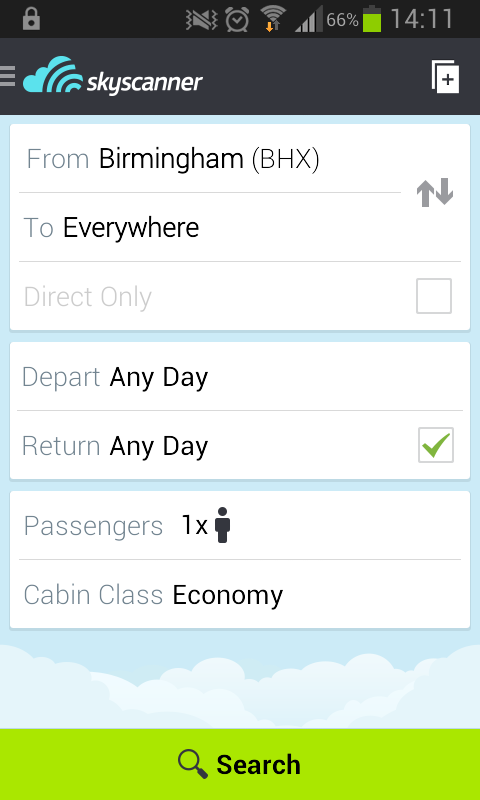
\includegraphics[width=\textwidth]{img/relatedReviews/SkyscannerFig1.png}
% 		\caption{Skyscanner's home screen}\label{fig:skyscannerfig1}
% 	\end{subfigure}%
% 	\qquad
% 	\begin{subfigure}[b]{0.2\textwidth}
% 		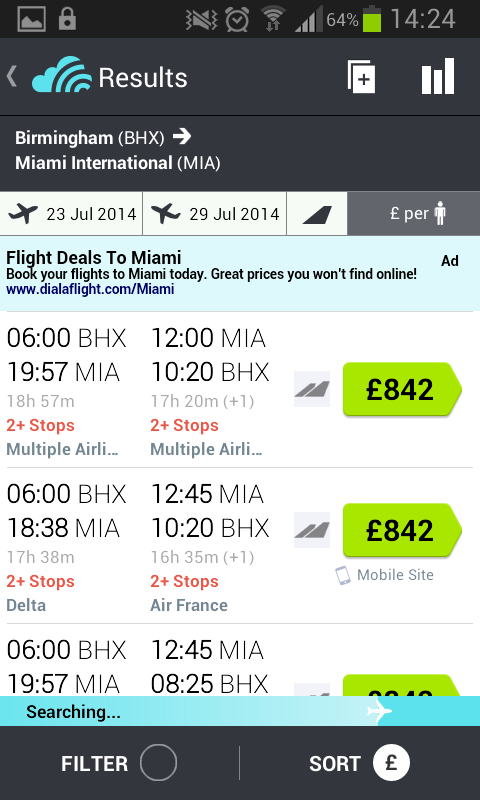
\includegraphics[width=\textwidth]{img/relatedReviews/SkyscannerFig2.png}
% 		\caption{Skyscanner's search results.}
% 	\end{subfigure}
% 	\caption{}\label{fig:skyscanner1}
% \end{figure}

\marginFig[0.8]{img/relatedReviews/SkyscannerFig2.png}{Skyscanner's search results
}{fig:skyscannerfig2}
\paragraph{Strengths}
\begin{itemize}
	\item The date selection page is simplistic and easy to use. The user is
		provided with a calendar where they can simply touch the date they
		would like to fly (figure~\ref{fig:skyscannerfig3}).
	\item Clear, concise information is shown on the results page. This allows
		the user to quickly scan the flights available and doesn't clutter the
		page with information which would not affect most customers' decisions
		(figure~\ref{fig:skyscannerfig2}). Further details (destinations and times
		of any stops) can be viewed by clicking on the flight.
	\item If a return date is not specified, an extra screen is displayed which
		allows the user to see the prices of different departure dates and the
		return dates available. This gives the customer an opportunity to
		change their departure date based on the prices shown.
		(figure~\ref{fig:skyscannerfig5})
	\item There is a filter option on the results page permitting users to be
		more specific. For example, particular airlines, direct flights only,
		flights times etc. (figure~\ref{fig:skyscannerfig4})
\end{itemize}
\begin{figure}[htbp]
	\centering
	\begin{subfigure}[b]{0.28\textwidth}
		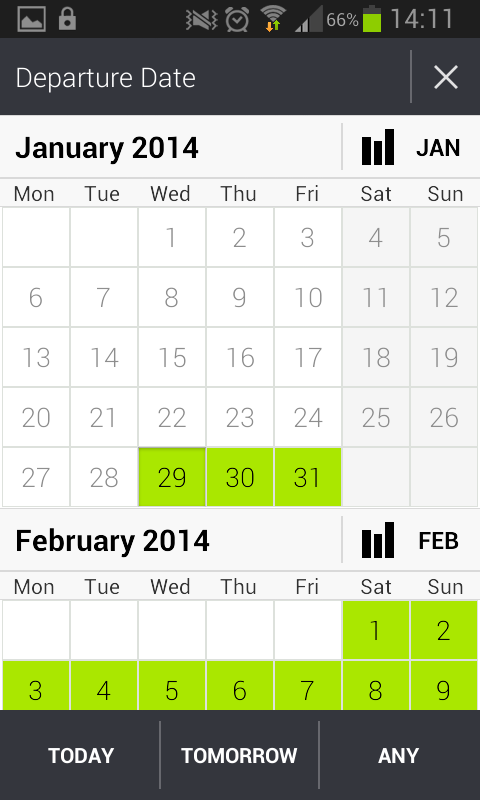
\includegraphics[width=\textwidth]{img/relatedReviews/SkyscannerFig3.png}
		\caption{Skyscanner's easy to use calendar for date selection.
		}\label{fig:skyscannerfig3}
	\end{subfigure}
	\qquad
	\begin{subfigure}[b]{0.28\textwidth}
		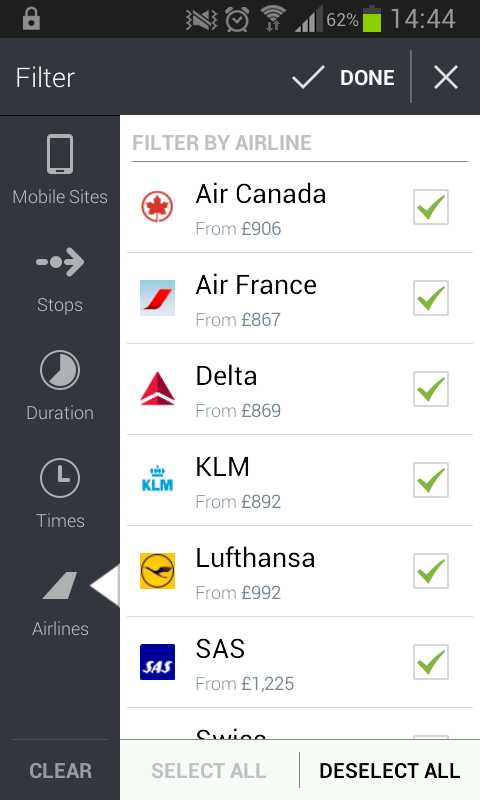
\includegraphics[width=\textwidth]{img/relatedReviews/SkyscannerFig4.png}
		\caption{Options available to further filter search results.
		}\label{fig:skyscannerfig4}
	\end{subfigure}
	\qquad
	\begin{subfigure}[b]{0.28\textwidth}
		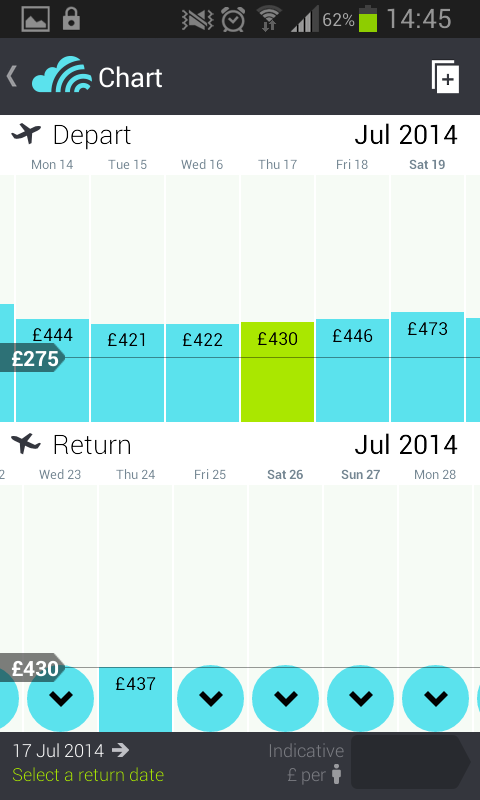
\includegraphics[width=\textwidth]{img/relatedReviews/SkyscannerFig5.png}
		\caption{Screen shows prices of alternative dates.
		}\label{fig:skyscannerfig5}
	\end{subfigure}
	\caption{}\label{fig:skyscanner2}
\end{figure}

\marginFig[0.8]{img/relatedReviews/SkyscannerFig1.png}{Skyscanner's home screen
}{fig:skyscannerfig1}
\paragraph{Weaknesses}
\begin{itemize}
	\item There is no flexibility in departure date (except for the option of
		``any'' date). However the return date option allows flexibility of one
		day.
	\item The ``Everywhere'' option (figure~\ref{fig:skyscannerfig1}) seems
		slightly pointless as it is unlikely someone would have no preference
		as to where they wish to go but have a particular date in mind. It is
		more likely they have a general idea of where they want to go, for
		example the country, but there is no option for this.
	\item When choosing a destination, the user is required to select a
		specific airport. This restricts the user to where they can fly. For
		example, they may wish to check prices to a variety of destinations
		within a particular area or group of Islands with various airports.
\end{itemize}

\subsubsection{Trivago}
\label{ssub:trivago}

Trivago is a hotel comparison website comparing hotels from booking sites such
as booking.com and Lastminute.com. The initial search screen boasts many
options and filters. As well as the expected search criteria such as location
and check in/out date, the user can also filter by rating, popularity,
distance, price and whether the hotel has certain features such as WiFi and a
pool etc. A maximum price and distance can also be set within a certain range
using the sliding bars (figures~\ref{fig:trivago1} and~\ref{fig:trivago1b}).
The results show the cheapest price for each hotel available and what booking
website the customer can get this price. Once the customer has chosen their
hotel, they will be directed to the booking website where they will make the
payment.
\marginFig[0.8]{img/relatedReviews/TrivagoFig1a.png}{Top half}{fig:trivago1}
\marginFig[0.8]{img/relatedReviews/TrivagoFig1b.png}{Bottom half}{fig:trivago1b}
% \begin{figure}[htbp]
% 	\centering
% 	\begin{subfigure}[b]{0.2\textwidth}
% 		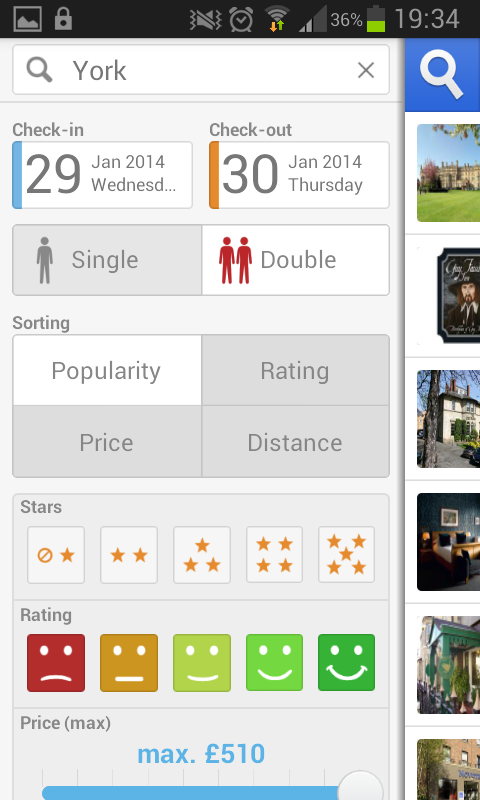
\includegraphics[width=\textwidth]{img/relatedReviews/TrivagoFig1a.png}
% 		\caption{Top half}
% 	\end{subfigure}
% 	\qquad
% 	\begin{subfigure}[b]{0.2\textwidth}
% 		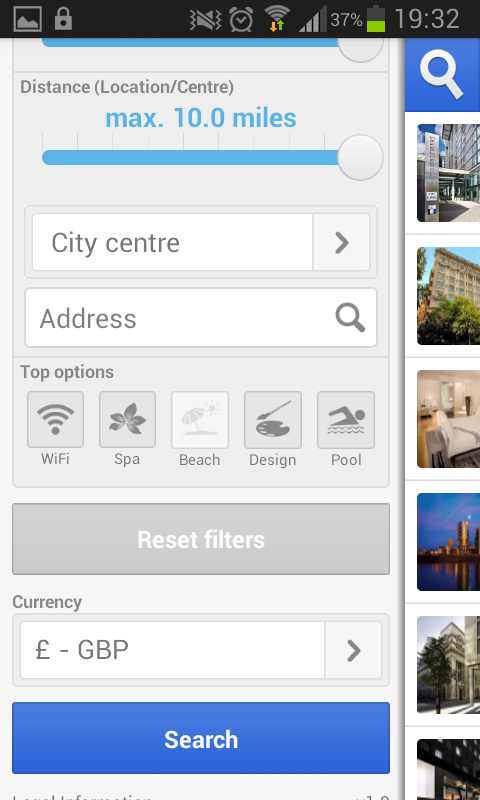
\includegraphics[width=\textwidth]{img/relatedReviews/TrivagoFig1b.png}
% 		\caption{Bottom half}
% 	\end{subfigure}
% 	\caption{Trivago's home screen}\label{fig:trivago1}
% \end{figure}

%TrivagoFig1a.png(home screen top half) TrivagoFig1b.png( home screen bottom half)

\paragraph{Strengths}
\begin{itemize}
	\item As a location is typed, the number of available hotels is displayed
		in brackets next to suggested locations.
	\item Searching is very flexible, for example you can search by hotel name,
		region, points of interest and city.
	\item It is possible to search for hotels in the vicinity of a specific
		address, very useful if you want to find the nearest hotel to a
		specific location.
	\item Search results automatically load up at the side of the screen as
		search criteria is filled out. The user can swipe across to see them,
		for example once a location had been entered, it will load up available
		hotels whilst still maintaining the search screen.
	\item The search results are very clear and simple in that they show enough
		information without clogging up the screen. The hotel name, rating,
		stars, distance from the centre, price and a photo are all displayed in
		a concise manner (figure~\ref{fig:TrivagoFig2}). The user can then look
		into more detail by clicking on the hotel
		(figure~\ref{fig:TrivagoFig3}).
\end{itemize}
\begin{figure}[htbp]
	\centering
	\begin{subfigure}[b]{0.33\textwidth}
		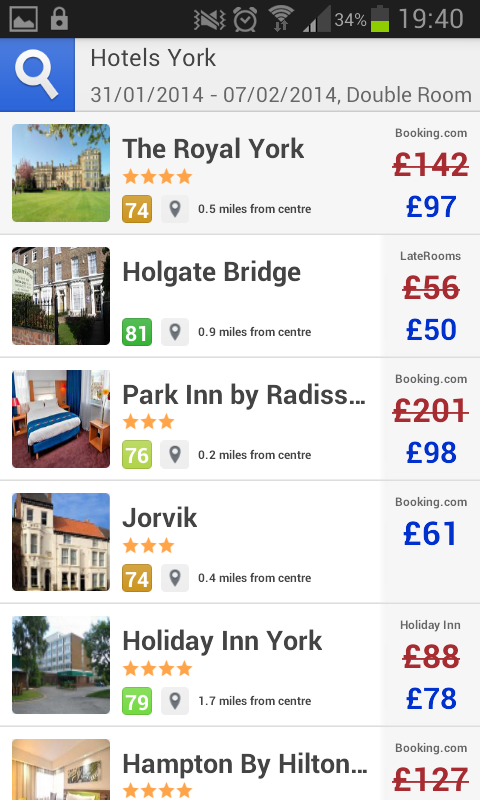
\includegraphics[width=\textwidth]{img/relatedReviews/TrivagoFig2.png}
		\caption{Trivago's earch results screen}\label{fig:TrivagoFig2}
	\end{subfigure}%
	\qquad
	\begin{subfigure}[b]{0.33\textwidth}
		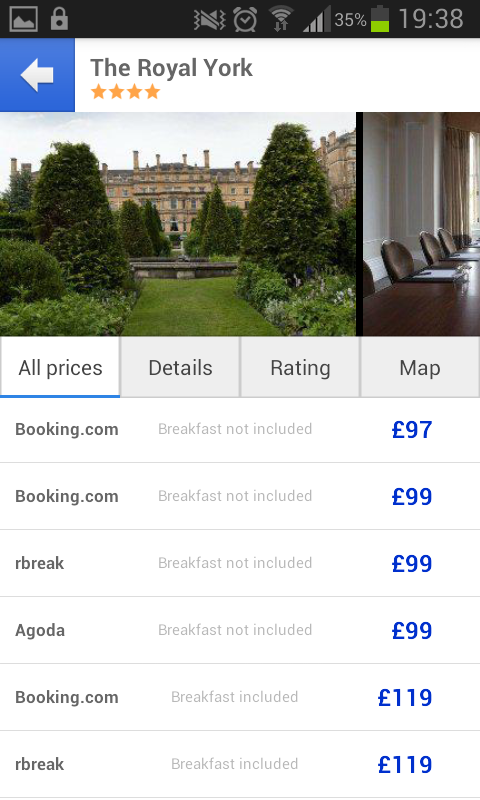
\includegraphics[width=\textwidth]{img/relatedReviews/TrivagoFig3.png}
		\caption{The hotel in more detail}\label{fig:TrivagoFig3}
	\end{subfigure}
	\caption{}\label{fig:trivago2}
\end{figure}

\paragraph{Weaknesses}

\begin{itemize}
	\item The `current location' feature in the search box is useful if you
		need a hotel there and then, but in reality this is rarely the case.
		Customers would usually book a hotel at least a day in advance at which
		point there current location is unlikely to be near an area they would
		need a hotel.
	\item There is no option to select how many people and therefore no option
		for multiple rooms. The user may require multiple rooms if there is
		more than two of them. Therefore this app is useless for families and
		people travelling in large groups.
	\item There are no additional filters past the home screen. Customers may
		require extra filters such as free parking.
\end{itemize}

\subsubsection{thetrainline.com}
\label{ssub:thetrainline}

thetrainline.com is a train ticket retailer app designed to let customers buy
train tickets without the need to have a paper ticket. This app differs
slightly in that it independently searches individual trains without searching
external websites. Train journeys can be searched by location of departure and
destination, departure/arrival  time and number of passengers, as shown in
figure~\ref{fig:theTrainLineFig1}. All available train journeys are then
displayed with the cheapest price for each journey.  Once the customer has
confirmed their chosen journey they can pay for their ticket on
thetrainline.com. The customer will be sent a barcode ticket to their mobile
phone.
% \begin{figure}[htbp]
% 	\centering
% 	\begin{subfigure}[b]{0.2\textwidth}
% 		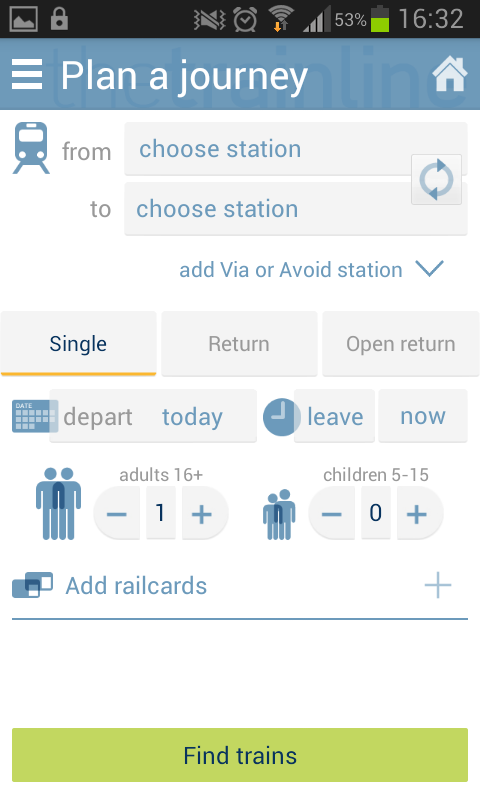
\includegraphics[width=\textwidth]{img/relatedReviews/theTrainLineFig1.png}
% 		\caption{Search criteria screen}\label{fig:theTrainLineFig1}
% 	\end{subfigure}%
% 	\qquad
% 	\begin{subfigure}[b]{0.2\textwidth}
% 		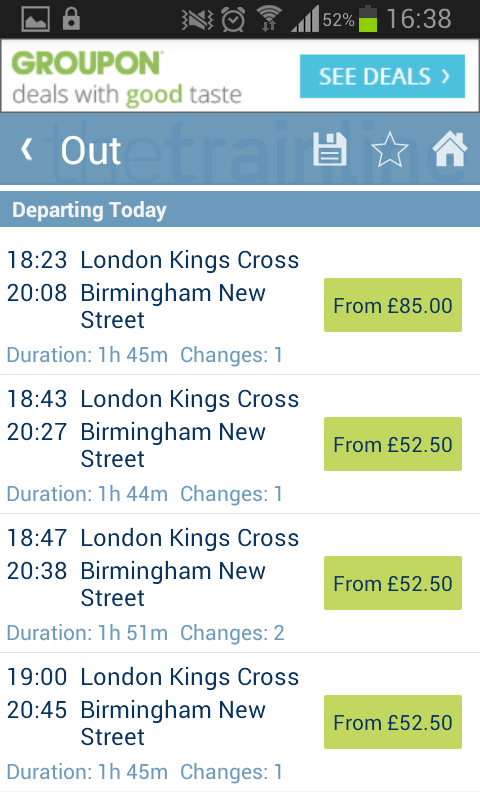
\includegraphics[width=\textwidth]{img/relatedReviews/theTrainLineFig2.png}
% 		\caption{Results from the search}\label{fig:theTrainLineFig2}
% 	\end{subfigure}
% 	\caption{Search using thetrainline.com application.
% 	}\label{fig:thetrainline1}
% \end{figure}
\marginFig[0.8]{img/relatedReviews/theTrainLineFig1.png}{thetrainline search criteria screen}{fig:theTrainLineFig1}
\marginFig[0.8]{img/relatedReviews/theTrainLineFig2.png}{Search results from thetrainline}{fig:theTrainLineFig2}

\paragraph{Strengths}

\begin{itemize}
	\item When typing the name of the station it suggests possible stations
		based on the first few letters. Useful if you're unsure of the name of
		the station. For example, typing `Birmingham' shows a list of all
		stations in Birmingham. In addition to this all recent searches are
		also displayed, so it is not necessary to type the name of the station
		each time.
	\item The app uses GPS to find the customers nearest station and it is also
		possible to set a home station to make it quicker and easier to plan a
		journey home every day. (figure~\ref{fig:thetrainline3})
	\item There is no redirection to another website, the customer can pay
		directly on thetrainline.com which provides a quicker and smoother
		payment process.
	\item The results shown are not limited to the specific time chosen,
		figure~\ref{fig:theTrainLineFig2}. This gives the customer an
		opportunity to choose an earlier or later train if it happens to be a
		lot cheaper.
\end{itemize}
\begin{figure}[htbp]
	\centering
	\begin{subfigure}[b]{0.33\textwidth}
		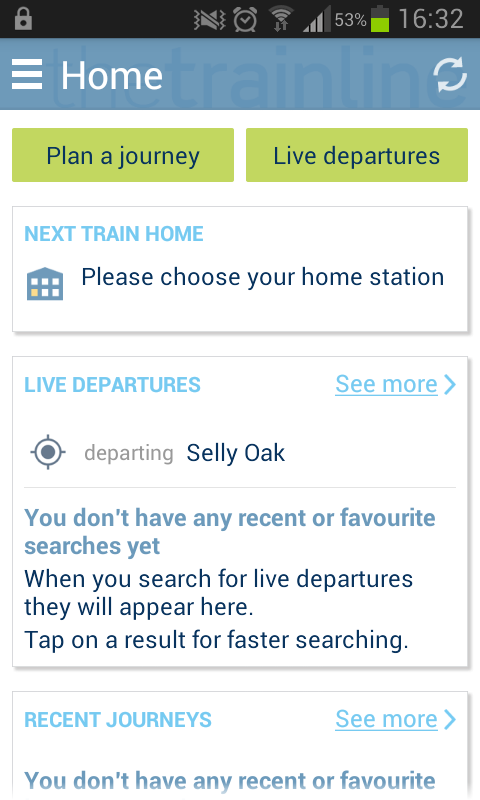
\includegraphics[width=\textwidth]{img/relatedReviews/theTrainLineFig3.png}
		\caption{Home screen showing GPS feature}
	\end{subfigure}%
	\qquad
	\begin{subfigure}[b]{0.33\textwidth}
		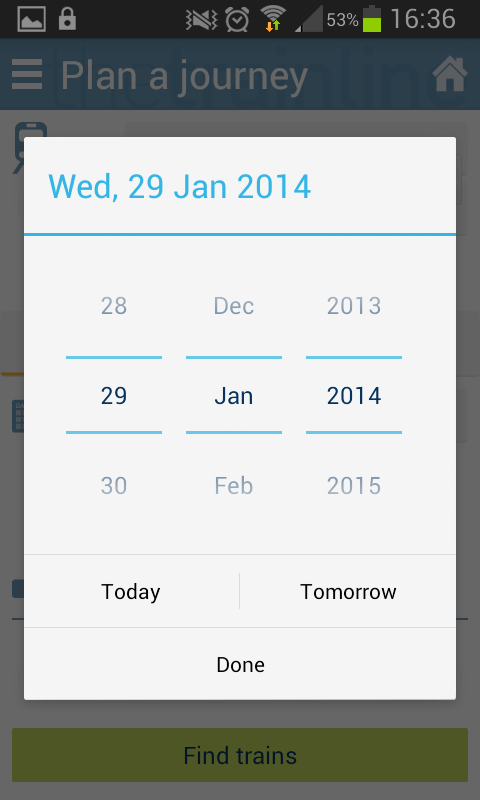
\includegraphics[width=\textwidth]{img/relatedReviews/theTrainLineFig4a.png}
		\caption{Sensitive time selection feature}
	\end{subfigure}
	\caption{}\label{fig:thetrainline3}
\end{figure}

\paragraph{Weaknesses}
\begin{itemize}
	\item The time and date selection feature is very sensitive and therefore
		requires a steady hand when scrolling up and down. The time can also be
		selected to the nearest minute, which when it comes to planning a
		journey, isn't particularly necessary considering multiple journeys are
		shown on the results page. Both these flaws contribute to time taken to
		find the desired journey.
\end{itemize}

\subsubsection{What we can learn}
\label{ssub:what_we_can_learn2}

\begin{itemize}
	\item Our sports booking app would benefit from having a GPS feature as
		those looking to play a particular sport would usually prefer to play
		near their current location. For the same reason, when the results are
		displayed, a filter for distance to the sport venue could be beneficial
		to the user.
	\item It would be useful if a message was sent to the users phone to
		confirm the booking. This will allow the user to check the booking
		details they are likely to forget such as court number or price. If the
		user booked the court well in advance, there could also be an option
		for the user to request  a reminder,  say a day before they are due to
		play.
	\item When searching for a particular location, the user should have the
		option to search by either postcode, address, town or city. By entering
		the city, this gives the user flexibility on location. However if the
		user does not wish to travel far, the other options would be more
		constructive. Either way, there is no restriction on how to search for
		a venue.
\end{itemize}
